\chapter[Dashboard]{Dashboard}
O objetivo deste capítulo é descrever a solução, a qual tem como objetivo atender às necessidades colocadas no primeiro capítulo, referente à problemática deste trabalho. A apresentação da solução está concentrada em três partes. A primeira parte está relacionada à coleta das métricas utilizando a ferramenta SonarQube, e a segunda parte está relacionada à criação do \textit{dashboard} e à visualização das informações. A terceira e última parte da solução, consiste na análise dos resultados obtidos através de uma avaliação qualitativa com possíveis usuários.

\section{Ambiente Simulado}
Para se simular um ambiente de produção, foi utilizado como modelo de referência o ambiente apresentado por Luiza e Yago \cite{luiza_yago}. No trabalho descrito, os autores caracterizam o Órgão pertencente à APF como Órgão X. Uma das características referentes ao Órgão X que podem ser citadas diz respeito a sua área de jurisdição que abrange serviços de radiodifusão, postais e de telecomunicações. O Órgão X atualmente implanta o GeDDAS (Gestão de Demandas de Desenvolvimento Ágil de Software) proposto por Souza \cite{souza_sobrinho_uso_2014}. A Figura \ref{img:proc_des} apresenta o processo de desenvolvimento adotado pelo Órgão X.

\graphicspath{{figuras/}}
\begin{figure}[h!]
\centering
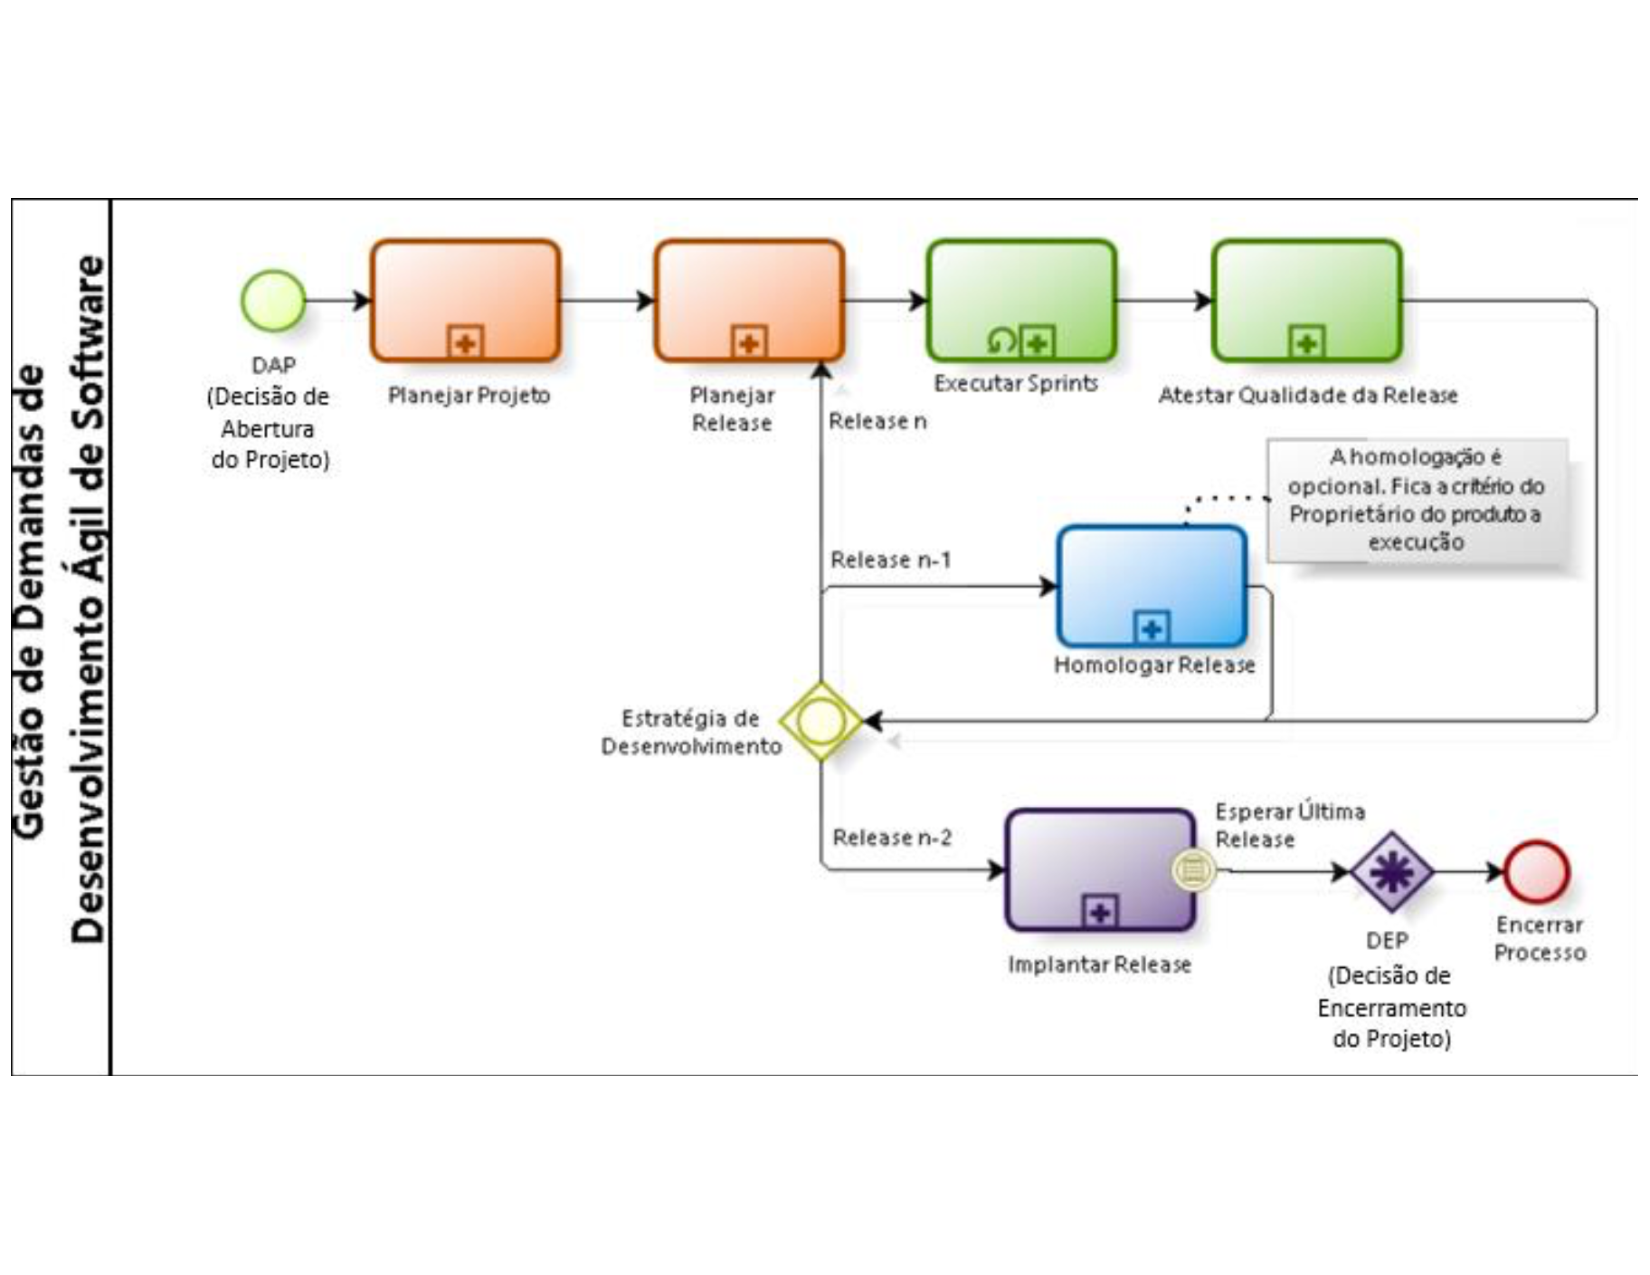
\includegraphics[scale=0.60]{Proc_des.pdf}
\caption{Processo de Desenvolvimento Adotado Pelo Órgão X. Fonte: \cite{luiza_yago}}
\label{img:proc_des}
\end{figure}

A solução tem o objetivo de atuar tanto do lado do Órgão Público, onde o Gestor acompanha o desenvolvimento do projeto, quanto da empresa contratada em que a ferramenta é integrada ao processo de desenvolvimento do software. A Figura \ref{img:ciclo_ver} apresenta um diagrama que demonstra o ciclo de verificação juntamente com a solução apresentada. Na Figura é possível observar que o time de desenvolvimento, da empresa contratada, desenvolve o código que é submetido para uma análise, onde é feita a verificação das métricas que foram estipuladas. Após essa análise o resultado é submetido para o \textit{dashboard},  dessa forma, tanto o Gestor de TI quanto a equipe de qualidade do Órgão, podem acompanhar o projeto. A figura \ref{img:diagram_implantacao} apresenta outra visão da integração entre a proposta e o ambiente de configuração do Órgão X.

\graphicspath{{figuras/}}
\begin{figure}[!]
\centering
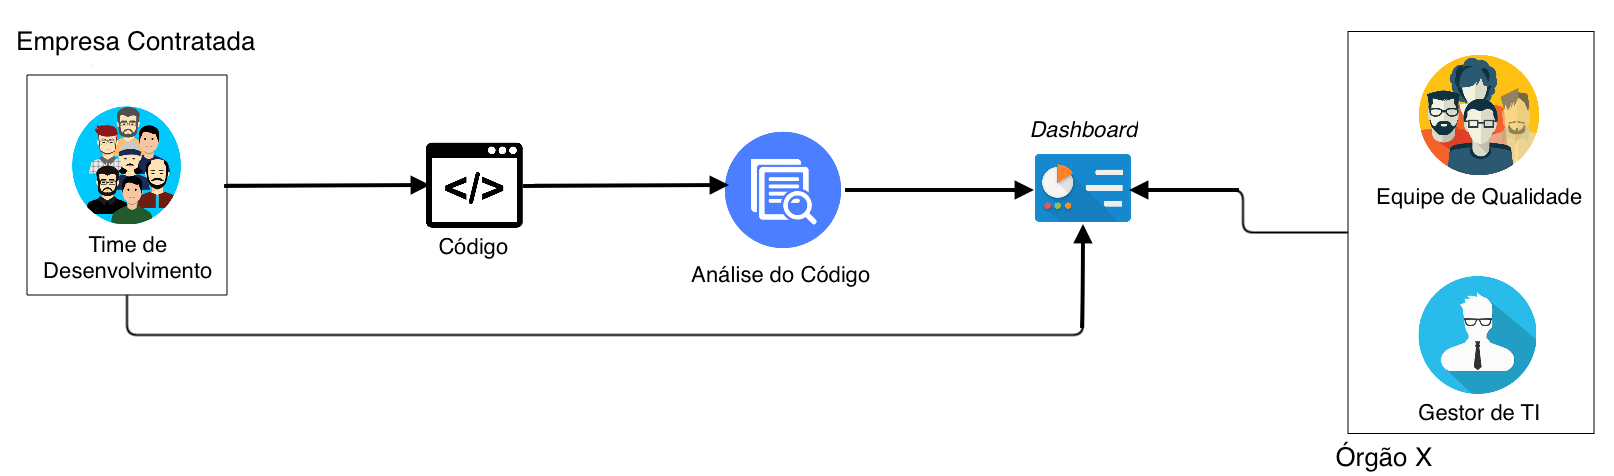
\includegraphics[scale=0.30]{proc_ver.png}
\caption{Ciclo de Verificação Utilizando a Solução Compartilhada Entre Órgão Contratante e Empresa Contratada}
\label{img:ciclo_ver}
\end{figure}

\graphicspath{{figuras/}}
\begin{figure}[!]
\centering
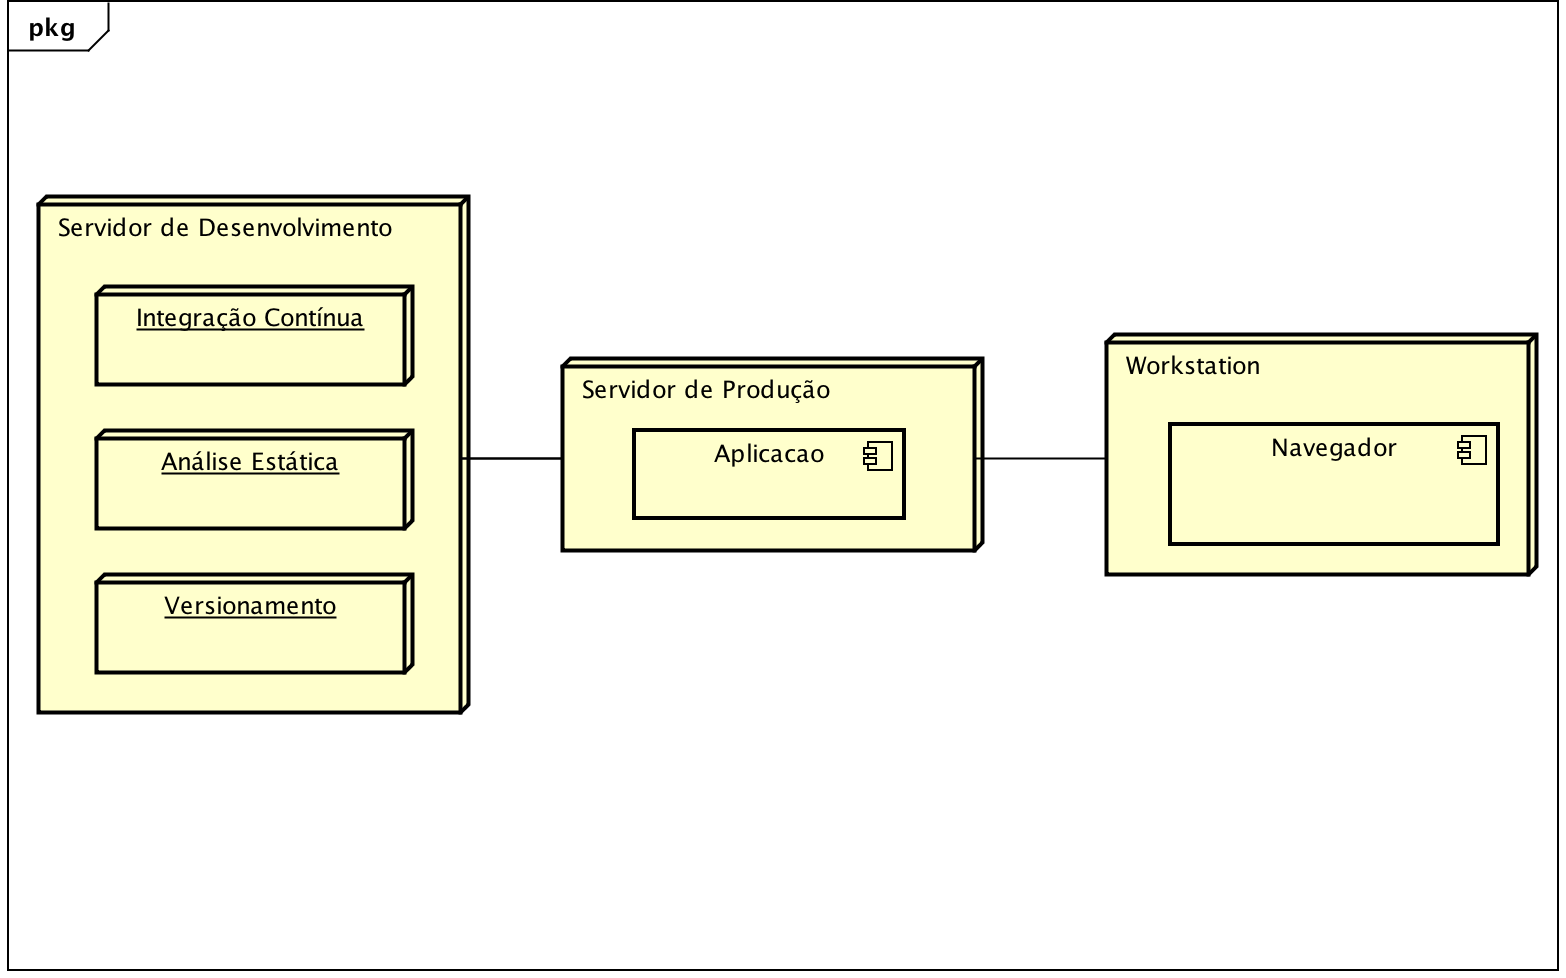
\includegraphics[scale=0.60]{diagrama_implantacao}
\caption{Diagrama de Implantação da Solução no Órgão X} 
\label{img:diagram_implantacao}
\end{figure}


\section{Coleta das Métricas}

Para fazer a coleta das métricas, foi utilizado a ferramenta SonarQube juntamente com a ferramenta Codacy como forma de elucidação de uma possível expansão que pode ser feita no software. Como já informado no capítulo de Suporte Tecnológico, a ferramenta Sonarqube é muito utilizada em Órgãos Públicos e em editais por ser uma ferramenta \textit{open-source}. Nesse contexto, a coleta das métricas é feita utilizando o SonarQube juntamente com o seu conjunto de métricas.

A sugestão das métricas utiliza o conceito do algoritmo de aprendizado de maquina, que sugere que o gestor avalie de 0 a 100, três métricas distintas de acordo com o quão necessário ele acredita ser aquela métrica para aquele projeto. Baseado nessa sugestão o algoritmo interpola os dados inseridos pelo usuário, juntamente com um conjunto de quatro \textit{Personas} com características específicas. Através do cruzamento dos perfis, o algoritmo sugere um conjunto de métricas baseado no perfil mais semelhante ao do usuário. A Figura \ref{img:perfis} apresenta de maneira simplificada como será o cruzamento dos dados entre as \textit{Personas} e o Usuário.

\graphicspath{{figuras/}}
\begin{figure}[h!]
\centering
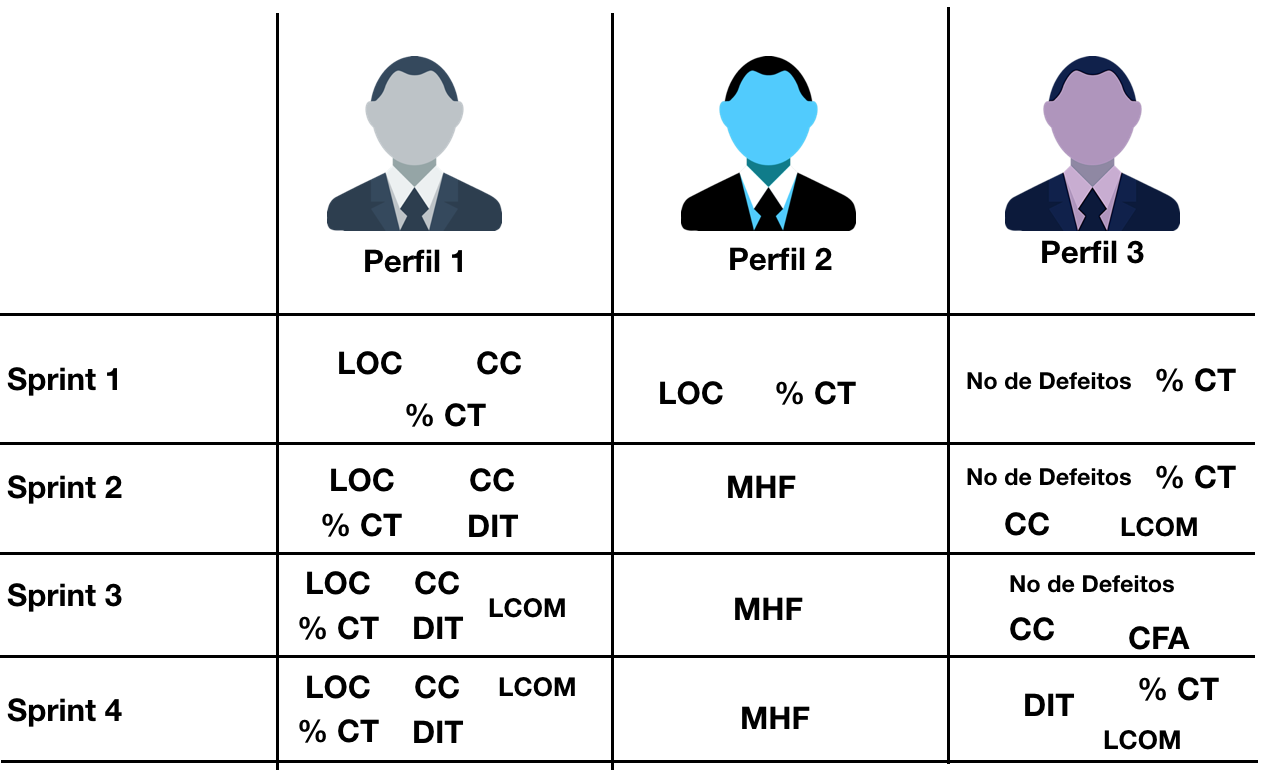
\includegraphics[scale=0.70]{perfis_exemplo.png}
\caption{Exemplo de Perfis Coletados Após Questionário}
\label{img:perfis}
\end{figure}

As métricas "Violações do tipo Blocker", "Violações do tipo Major" e "Violações do tipo Minor" são estipuladas de acordo com o próprio perfil do Sonar, chamado Sonar Way. Contudo, a melhor maneira seria criar um perfil com as regras da própria organização garantindo uma avaliação mais focada no objetivo do Órgão.


O objetivo deste trabalho é criar uma ferramenta que auxilie na auditoria de produtos de software entregues por empresas terceirizadas. Entretanto dificilmente o mesmo irá substituir o fator humano da auditoria. Portanto, o software compreende apenas um suporte, que visa facilitar a avaliação geral do software entregue sob o ponto de vista da qualidade de código. Recomenda-se que o software seja submetido à ferramenta e seja aceito, a realização de uma auditoria em cima de uma amostragem do software entregue, sob o olhar de um analista especializado para tal atividade.

Foi elaborado uma prova de conceito, para que se pudesse testar a funcionalidade relacionada à coleta de métricas. Está prova, consiste em, elaborar um software que fosse capaz de extrair métricas do relatório do SonarQube. Inicialmente foi necessário criar uma instância do SonarQube e fazer a análise de um projeto. O projeto escolhido foi um projeto em Java, que o próprio SonarQube disponibiliza para download, com o intuito de ser utilizado como exemplo. Com o ambiente configurado, implementou-se uma solução em Python que atendesse aos requisitos estabelecidos para a prova de conceito. A Figura \ref{img:terminal} apresenta a saída do console, ao se rodar a solução.


\graphicspath{{figuras/}}
\begin{figure}[H]
\centering
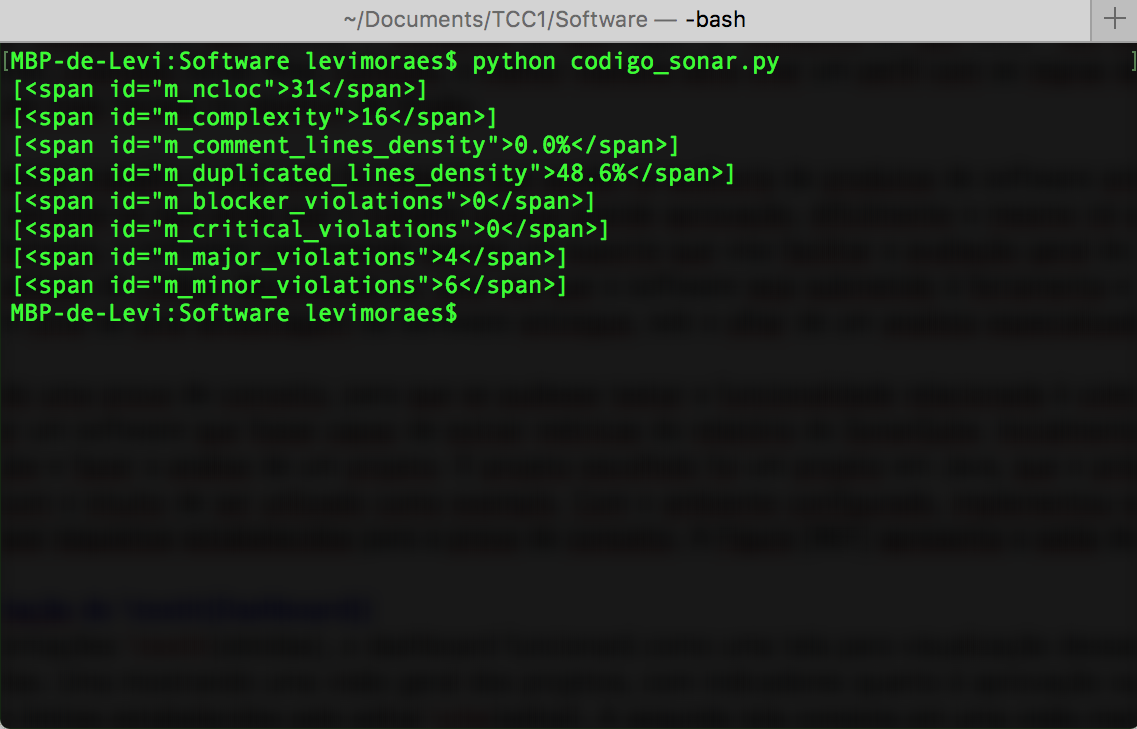
\includegraphics[scale=0.60]{terminal.png}
\caption{Métricas Extraídas do SonarQube}
\label{img:terminal}
\end{figure}

Na primeira linha da Figura \ref{img:terminal}, é executada a chamada do código. As linhas seguintes apresentam as métricas coletadas pela solução. As métricas que são apresentadas no console, foram definidas no código, por este motivo, ainda não é possível definir outras métricas durante a execução da aplicação, esta funcionalidade será implementada na segunda fase do projeto. 

\section{Criação do \textit{Dashboard}}

O principal objetivo do dashboard é facilitar a visualização de um conjunto de métricas que podem ser obtidos de várias fontes. A solução é composta por duas telas. Uma mostrando uma visão geral dos projetos, com indicadores quanto ao estado atual do projeto. A segunda tela consiste em uma visão mais detalhada sobre cada projeto, mostrando a evolução do projeto em cada métrica e com um \textit{link} para o Sonar de cada métrica para um aprofundamento.

Para melhor compreensão da proposta, foram elaborados protótipos das possíveis telas que farão parte da solução final. A Figura \ref{img:telaLogin} apresenta a tela inicial da solução, por onde o Gestor fará o acesso colocando seu \textit{username} e seu \textit{password}. Ainda nesta tela, existe um \textit{link} para caso o Gestor não se lembre do seu \textit{password}, onde o sistema enviará uma mensagem, para o \textit{email} cadastrado, solicitando a alteração.

\graphicspath{{figuras/}}
\begin{figure}
\centering
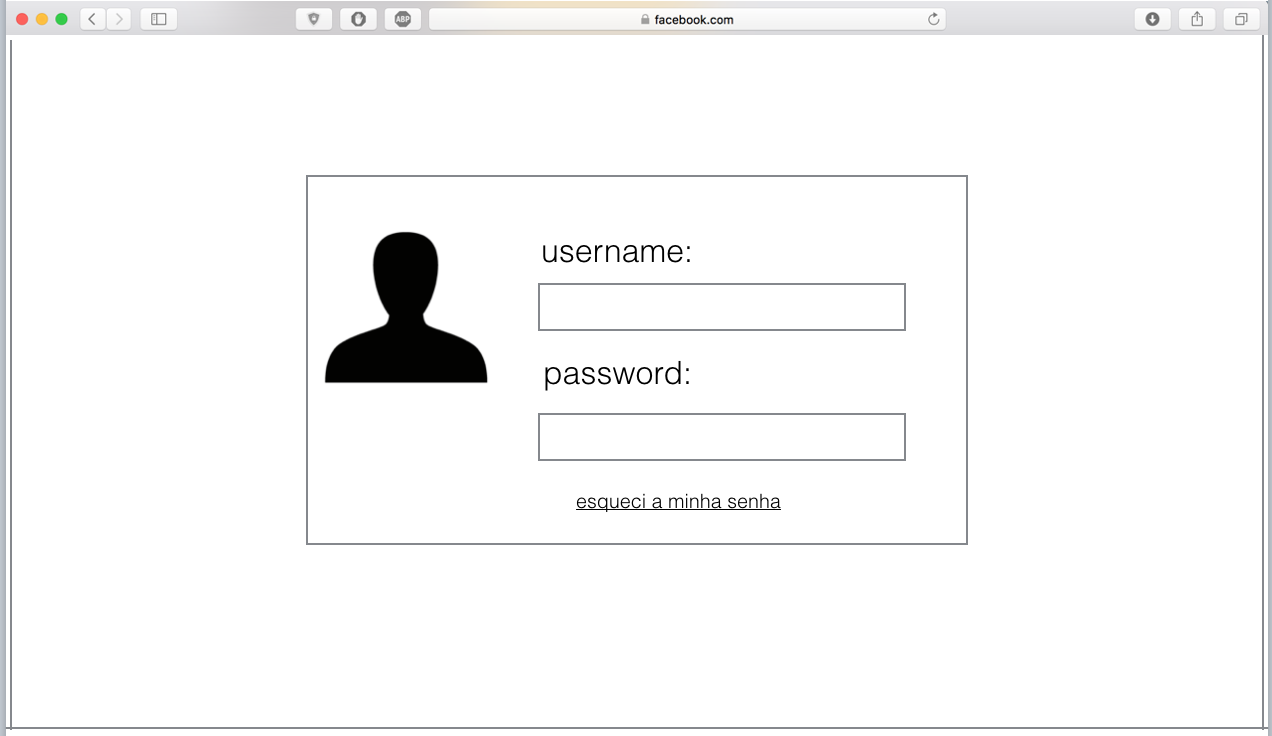
\includegraphics[scale=0.60]{telaLogin.png}
\caption{Tela Login}
\label{img:telaLogin}
\end{figure}

A página inicial da solução, também chamada de \textit{home page}, aqui apresentada na Figura \ref{img:telaHome}. Nesta página, o Gestor tem uma visão de todos os projetos, que ele cadastrou para serem acompanhados. Cada projeto é representado por um retângulo de uma cor , e neste retângulo estão algumas informações referentes ao projeto, que podem ser visualizadas, sem a necessidade de se abrir o projeto. Tanto as cores dos retângulos, como as informações dos projetos podem ser customizadas de acordo com o Gestor. Nesta página, ainda existe um botão que direciona o usuário para a tela de "adicionar projetos". Esta tela é somente para o gestor.
 
\graphicspath{{figuras/}}
\begin{figure}
\centering
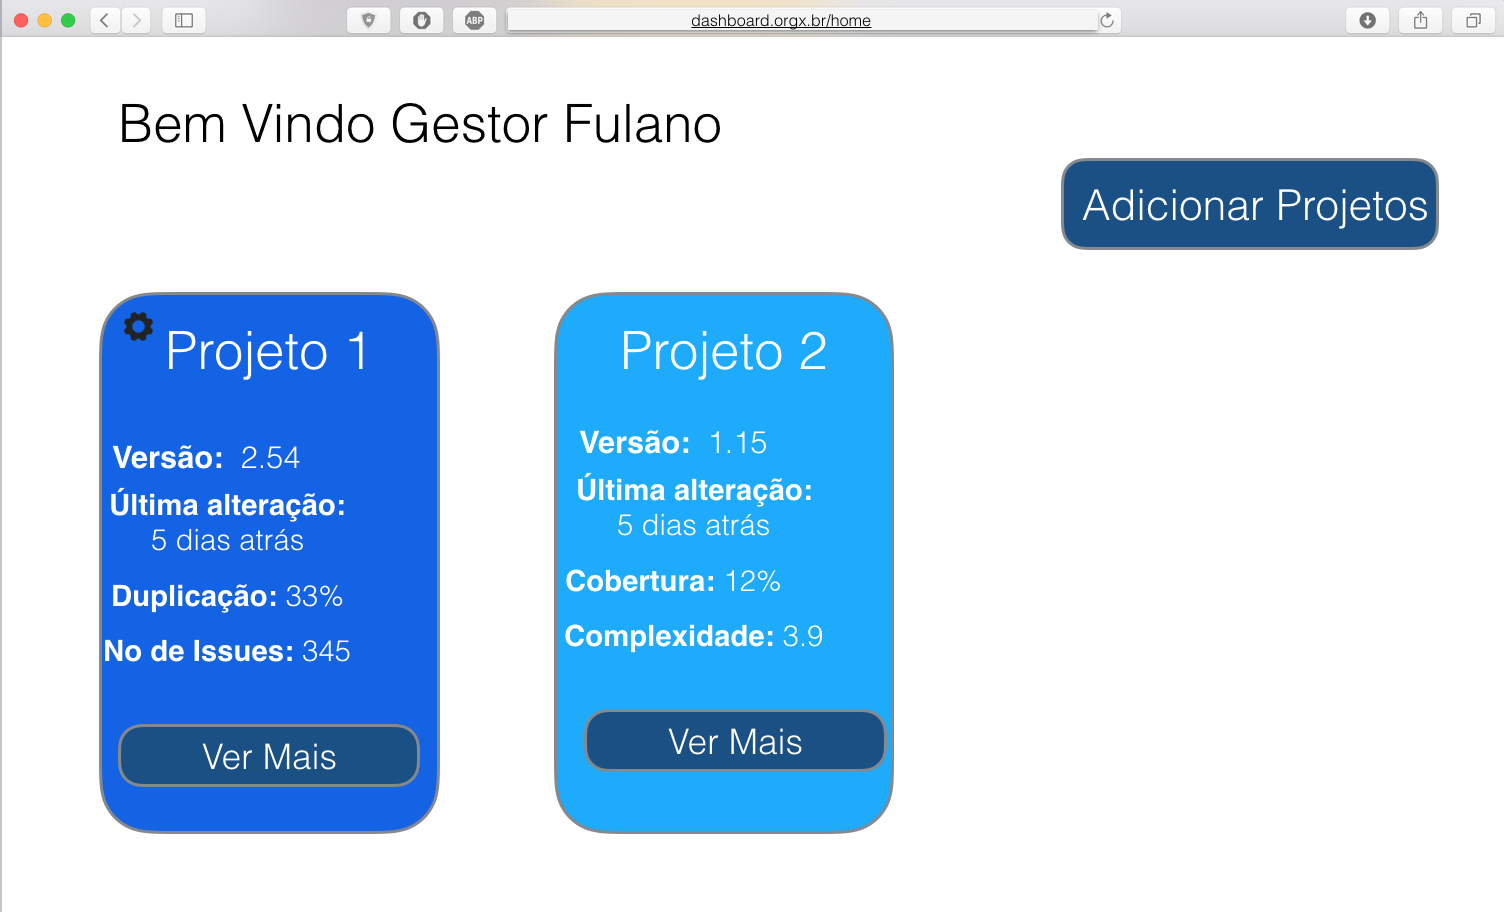
\includegraphics[scale=0.60]{telaHome2.png}
\caption{Tela Home}
\label{img:telaHome}
\end{figure} 

A Figura \ref{img:telaDashboard} apresenta um protótipo do \textit{dashboard} que será implementado. Nesta página encontram-se as informações referentes ao projeto selecionado. Está página apresenta em forma de gráficos, as métricas que foram selecionadas pelo Gestor para aquele projeto. Esta é a única página que pode ser acessada pela empresa terceirizada. Em cada métrica é possível passar colocar a seta do \textit{mouse} por cima do ícone "?" para que se tenha uma breve explicação da métrica 

\graphicspath{{figuras/}}
\begin{figure}
\centering
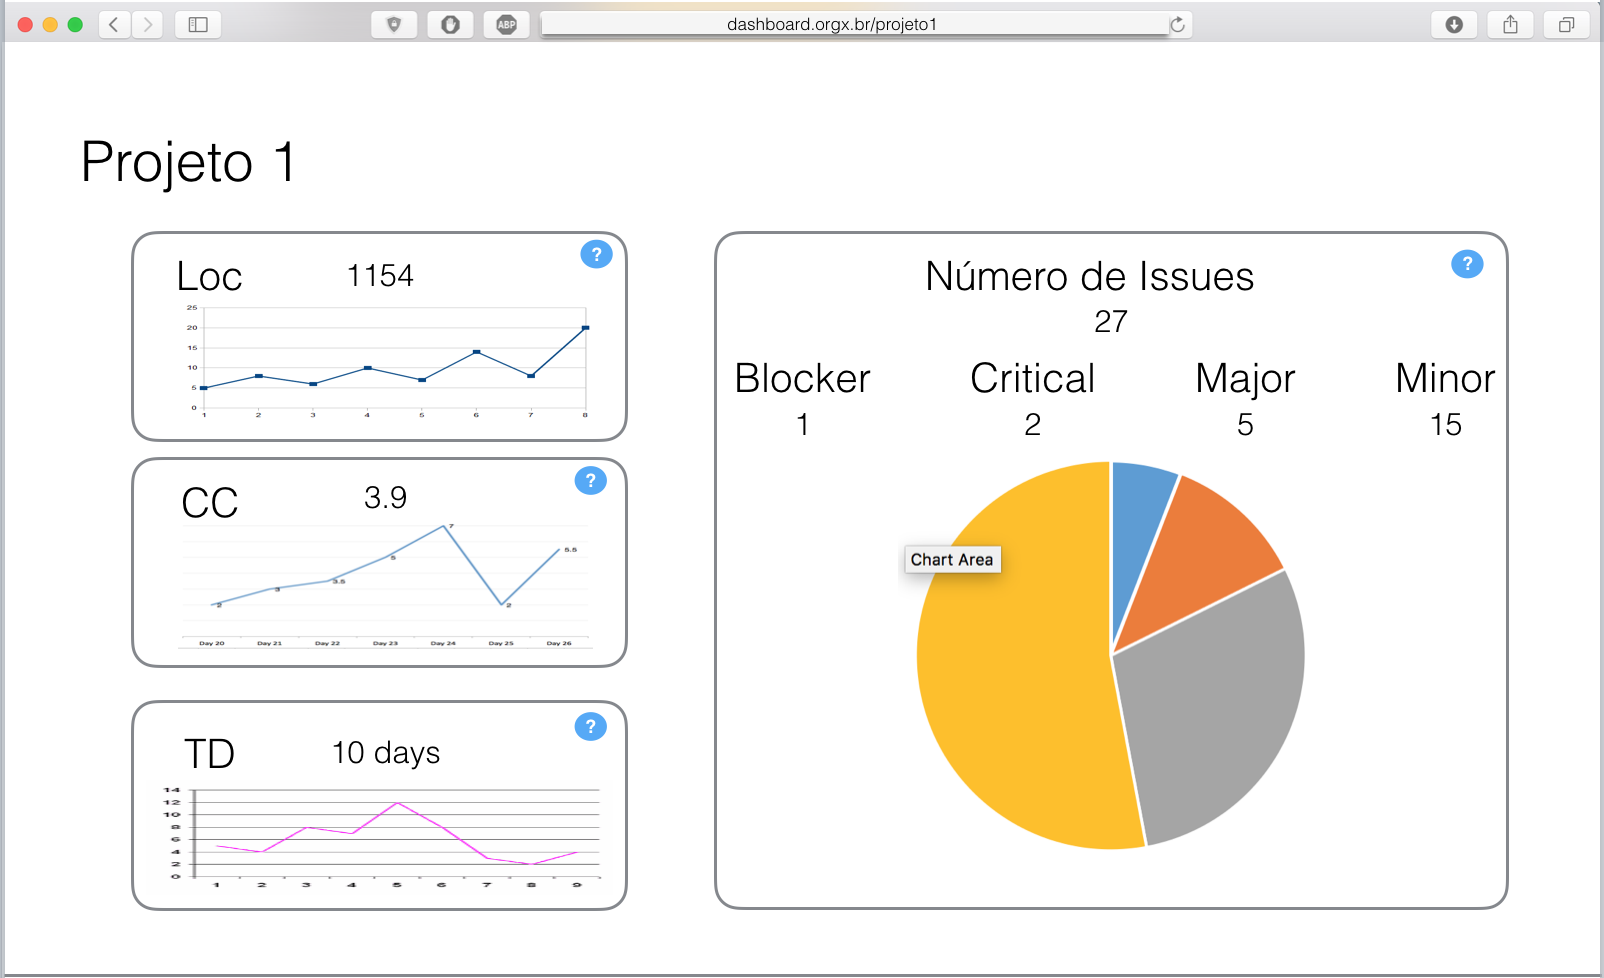
\includegraphics[scale=0.60]{telaDashboard.png}
\caption{Tela Dashboard}
\label{img:telaDashboard}
\end{figure} 

Para se fazer a adição de um novo projeto, é necessário que o projeto a ser adicionado, esteja armazenado em um repositório que o Gestor tenha acesso de leitura. A Figura \ref{img:telaAdicionar} representa um protótipo da página de adição de projetos. Nesta página são adicionados, o nome do projeto, uma descrição, a url do repositório em que se encontra o projeto e por último, as métricas que serão analisadas. Assim como na página do \textit{dashboard}, cada métrica apresenta um ícone "?" que apresenta uma breve explicação de cada métrica.

\graphicspath{{figuras/}}
\begin{figure}
\centering
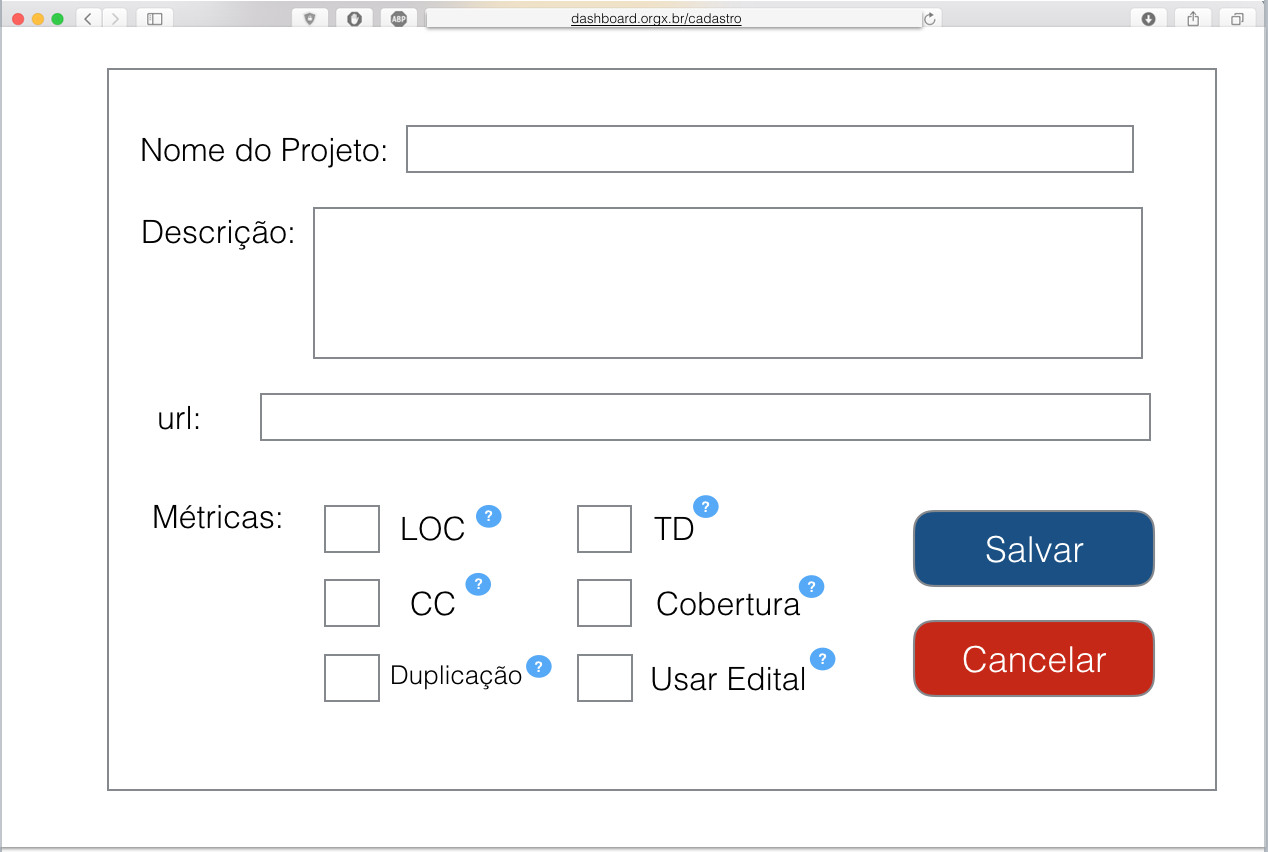
\includegraphics[scale=0.60]{telaAdicionar.png}
\caption{Tela Adicionar}
\label{img:telaAdicionar}
\end{figure} 

Assim como a coleta de métricas, também foi elaborada uma prova de conceito, para testar a exibição dos gráficos que seriam mostrados no \textit{dashboard}. Esta era uma continuação da prova de conceito da coleta de métricas, em que, feita a coleta, deveria-se exibir as métricas em um gráfico. A Figura \ref{img:dashboard} apresenta a tela relacionada à esta prova de conceito.

\graphicspath{{figuras/}}
\begin{figure}[H]
\centering
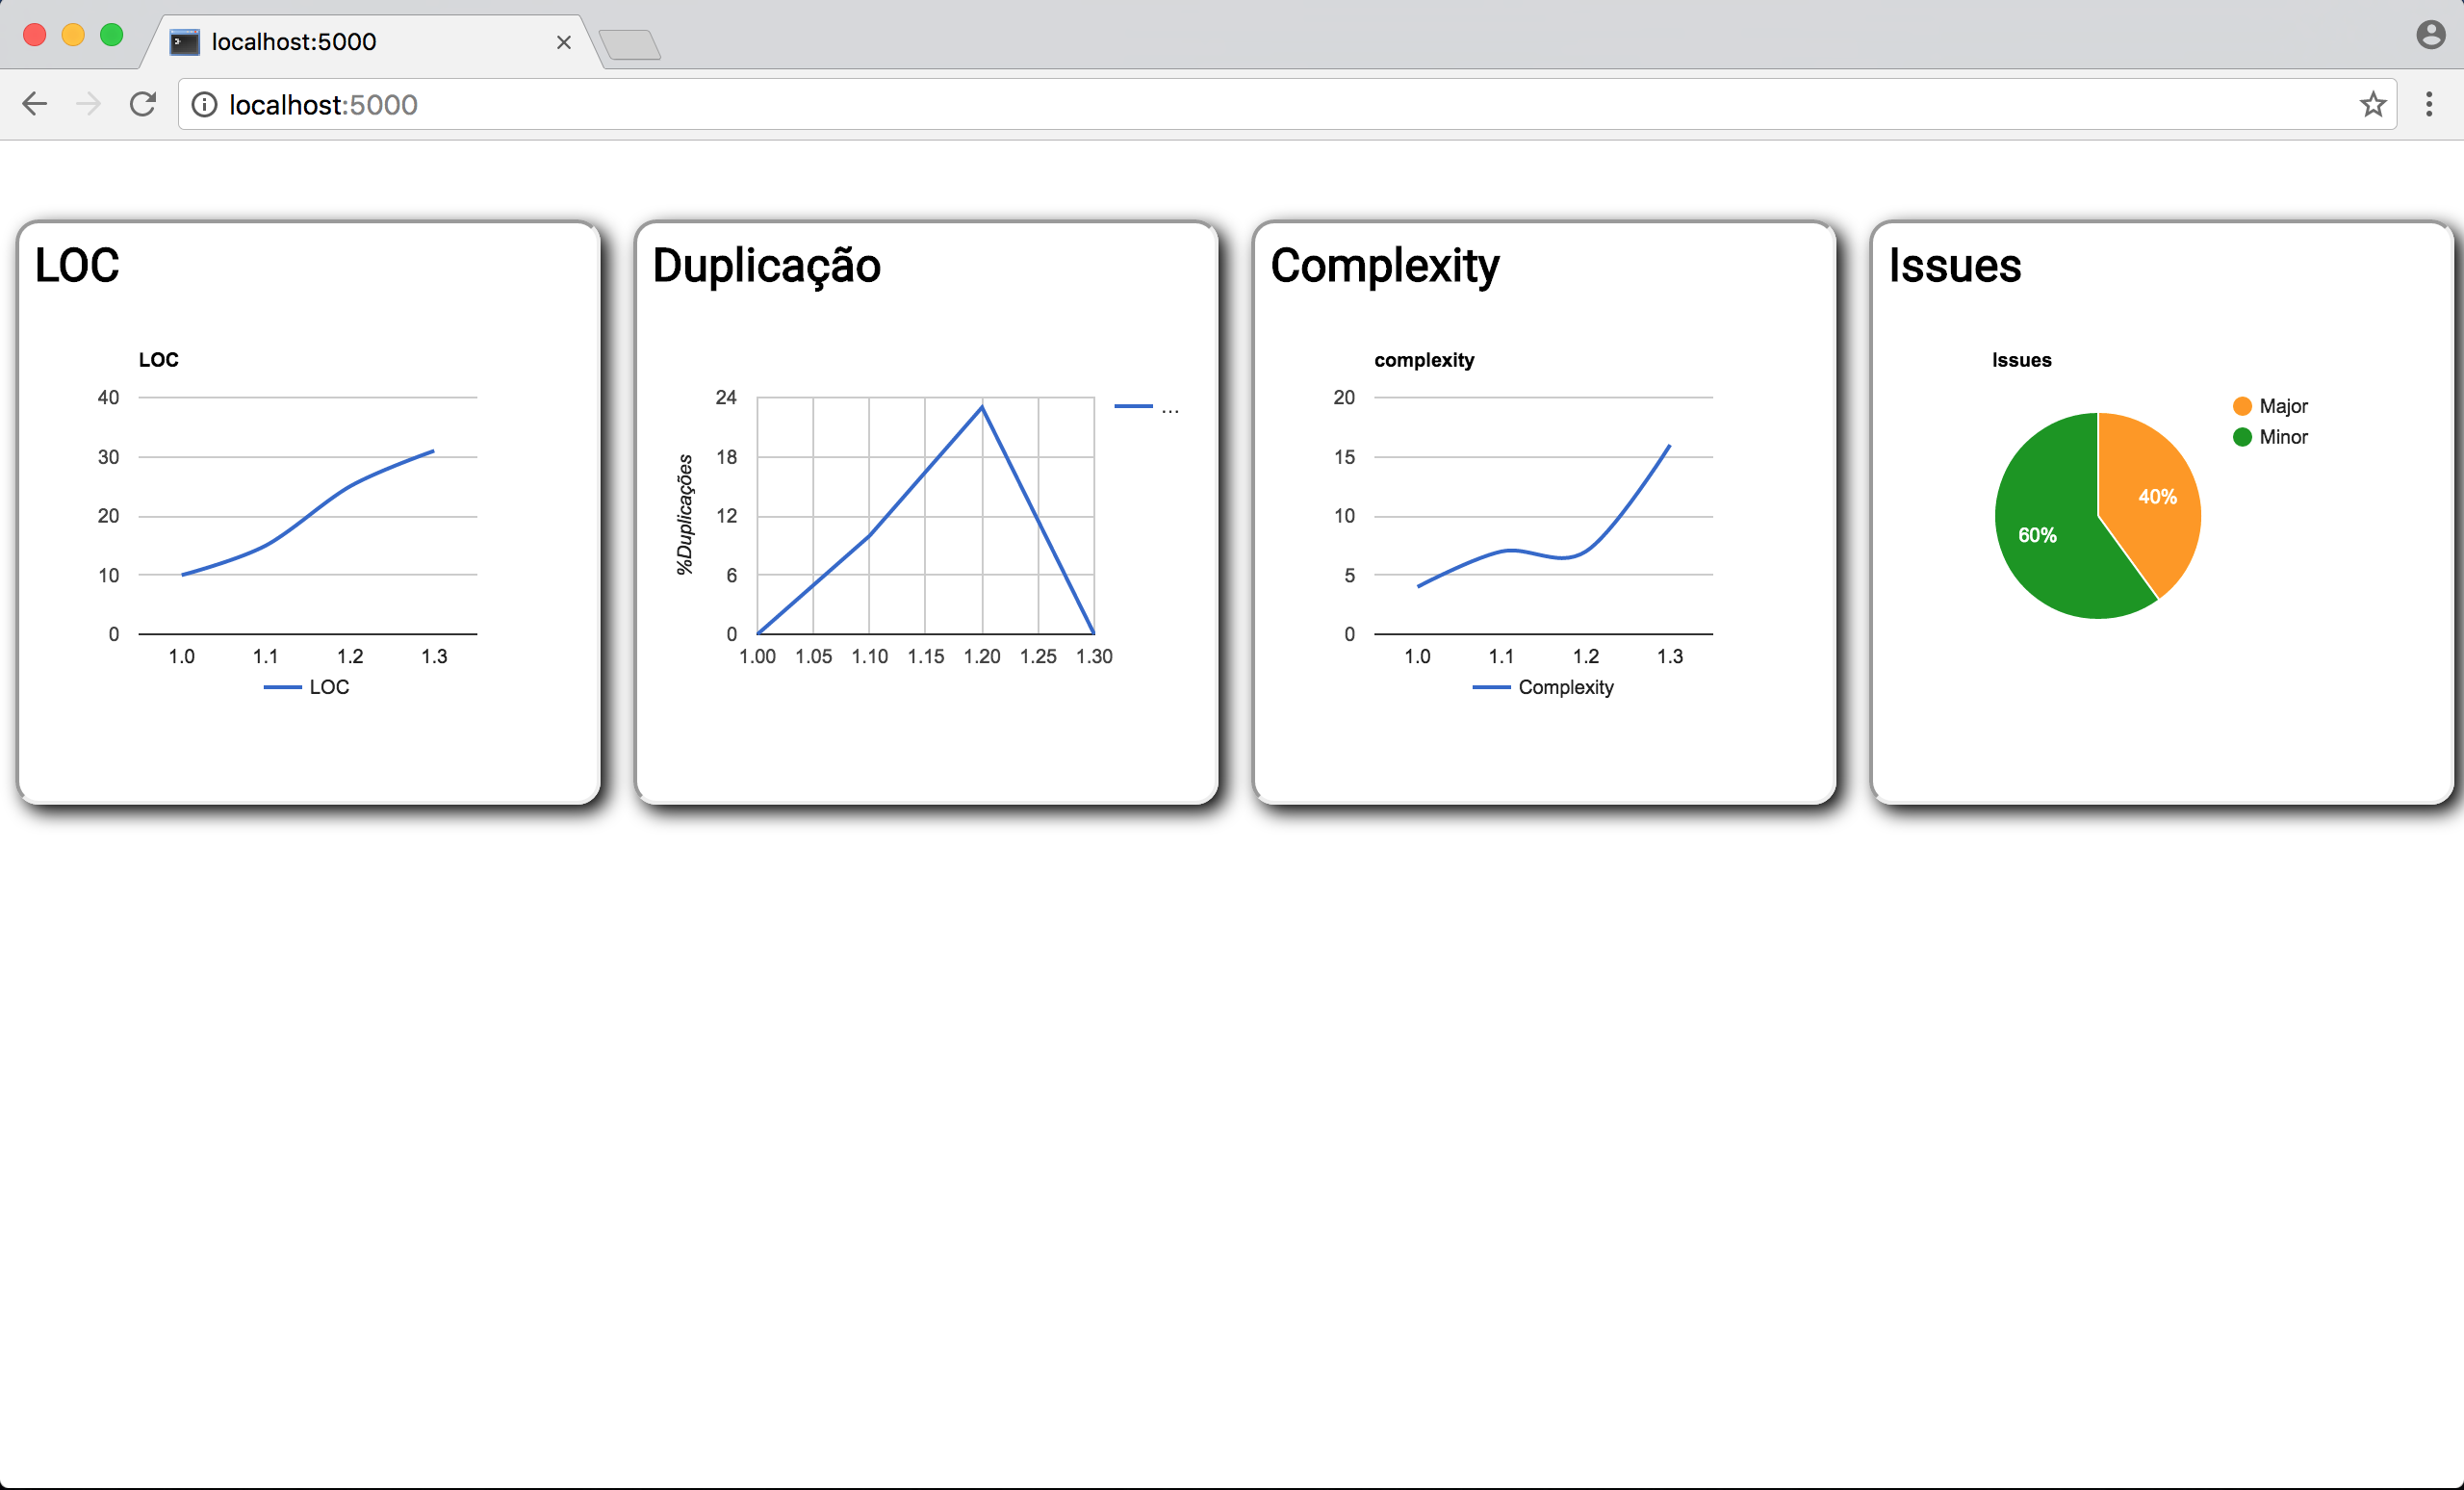
\includegraphics[scale=0.35]{dashboard_conceito.png}
\caption{Página do \textit{Dashboard} da Prova de Conceito}
\label{img:dashboard}
\end{figure}

\section{Avaliação}

A avaliação do \textit{dashboard} foi feita por parte de um gestor de tecnologia de um Órgão Público. Essa avaliação será conduzida em um período de três iterações e com sete gestores. Nestas iterações serão avaliados aspectos de usabilidade da ferramenta e se a ferramenta possuiria condições mínimas de ser implantada. Caso não seja possível essa avaliação com um profissional da área, as avaliações serão feita através de alunos ou professores que possuem tal experiência com contratação de software para Órgãos Públicos, novamente avaliando aspectos como usabilidade e melhorias necessárias para implantação em um Órgão. Na última iteração será pedido aos entrevistados que respondam a um questionário elaborado segundo o modelo do SUS. O objetivo dessa avaliação é para que se tenha quantificado o nível de usabilidade do software entregue.


\section{Resumo do Capítulo}

A proposta deste trabalho é criar uma maneira facilitada de acompanhar a qualidade de código estático dos produtos de software entregues pelas tercerizadas. Para fazer esta análise, a solução orienta-se por uma ferramenta de análise estática SonarQube e por um conjunto de métricas relacionadas às boas práticas de programação encontradas na ferramenta Codacy. A solução encontrada é a utilização de um \textit{dashboard} que através de um algoritmo de sugestão, auxilie o gestor no acompanhamento de um projeto, e que através dessas métricas, seja possível aferir a qualidade do código para aquelas métricas. A última etapa deste trabalho, consiste em conjunto de testes de usabilidade feitos juntamente com gestores de projeto, ou caso não seja possível, com professores e alunos. Durante três iterações serão avaliados aspectos de usabilidade e aplicabilidade da solução proposta em um ambiente real.